% vim: set fenc=utf-8 ft=latex encoding=utf-8
% -*- mode: latex; coding: UTF-8; -*-

\newif\ifdraft
\drafttrue

\ifdraft
        \documentclass[conference, draftclsnofoot]{IEEEtran}
        \def\baselinestretch{1}
        \setlength{\marginparwidth}{2cm}
\else
        \documentclass[conference]{IEEEtran}
        \def\baselinestretch{1}
        \setlength{\marginparwidth}{2cm}

        % \documentclass[conferece, final]{IEEEtran}
\fi

\usepackage[T1]{fontenc}
\usepackage[utf8]{inputenc}

\newcommand{\TheTitle}{Visualizing Release Information of Linux}
\newcommand{\TheAuthors}{Evan Wilde}
\newcommand{\TheEmails}{etcwilde@uvic.ca}
\newcommand{\TheSubject}{Digesting large amounts of commit data}
\newcommand{\TheKeywords}{Linux, git, data structures, tree data structures}

\synctex=1

\usepackage[hyphens]{url}
\urlstyle{same}

\ifdraft
        \usepackage[unicode=true,bookmarks=false,breaklinks=false,
                pdfborder={0 0 0},backref=none,colorlinks=true]{hyperref}

\else
        \usepackage[unicode=true,bookmarks=false,breaklinks=false,
                pdfborder={0 0 0},backref=none,colorlinks=false]{hyperref}
\fi

\usepackage[nospace]{cite}

% Table Support
\usepackage{dcolumn}
\usepackage{longtable}

\usepackage{balance}
\usepackage{placeins}
\usepackage{multirow}

% Extra support
\usepackage{xspace}
\usepackage{caption}
\usepackage[nospace]{cite}

% Fix any bad-hyphenations here
\hyphenation{}

% \ifdraft
%     \usepackage[colorinlistoftodos]{todonotes}
%     \newcommand{\evan}[1]{{\color{blue}\emph{Evan Says: #1}}\xspace}
%     \newcommand{\evantodo}[1]{{\color{blue}\emph{Evan Todo: #1}}\xspace}
%     \newcommand{\dmg}[1]{{\color{blue}\emph{dmg Says: #1}}\xspace}
%     \newcommand{\dmgtodo}[1]{{\color{blue}\emph{dmg Todo: #1}}\xspace}
% \else
%     \usepackage[disable]{todonotes}
%     \newcommand{\evan}[1]{}
%     \newcommand{\evantodo}[1]{}
%     \newcommand{\dmg}[1]{}
%     \newcommand{\dmgtodo}[1]{}
% \fi
    \usepackage[colorinlistoftodos]{todonotes}

\newcommand{\tool}{{\emph Linvis}\xspace}


    \newcommand{\evan}[1]{{\color{blue}\emph{Evan Says: #1}}\xspace}
    \newcommand{\evantodo}[1]{{\color{blue}\emph{Evan Todo: #1}}\xspace}
    \newcommand{\dmg}[1]{{\color{blue}\emph{dmg Says: #1}}\xspace}
    \newcommand{\dmgtodo}[1]{{\color{blue}\emph{dmg Todo: #1}}\xspace}


%%% Local Variables:
%%% mode: plain-tex
%%% TeX-master: t
%%% End:


\begin{document}

\title{\TheTitle}
\author{
\IEEEauthorblockA{\TheAuthors}
\IEEEauthorblockN{Department of Computer Science,
                    University of Victoria, Canada.}
\IEEEauthorblockA{Email: \TheEmails}
}
\maketitle
\begin{abstract}

        With an average of more than 900 top-level merges into the Linux kernel per
        release, many containing hundreds of commits and some containing thousands,
        maintenance of older versions of the kernel becomes nearly impossible.
        Various commercial products, such as the Android platform, run older
        versions of the kernel. Due to security, performance, and changing hardware
        needs, maintainers must understand how updates made to the current version
        of the kernel fit into older versions in order to make the necessary
        patches.

        Current tools provide information about repositories through the directed
        acyclic graph (DAG), which is helpful for smaller projects. However with the
        scale and number of branches in the kernel the DAG becomes overwhelming very
        quickly.

        In this paper, we present a tool that uses a tree-based model, as described
        by German et al., to construct a clearer summary of the changes made. This
        tool is designed to allow users to explore the topology of the repository
        for a given release of the kernel and view an aggregated summary of the
        changes made.

\end{abstract}

\begin{IEEEkeywords}
\TheKeywords
\end{IEEEkeywords}

\section{Introduction}

Maintainers of older versions of the Linux kernel must sift through thousands of
commits with tools that are unable to filter and effectively visualize projects at
the scale of the kernel. Tools like Gitk use a directed acyclic graph (DAG) model,
showing all commits and merges in chronological order by when the commit was
authored. This representation works in smaller projects; it enables users to see
when changes are made, when these changes are merged, and how each branch is
interacting.  In large modular projects, like the Linux kernel, the DAG becomes a
mess of merges and commits (figure \ref{fig:gitk}) losing its visual meaning. In
some cases, the Linux kernel is simply too large for the system to generate a
visualization. Github provides a DAG view for many projects, but is unable to
display the visualization for projects as large as the Linux kernel (figure
\ref{fig:gitfail}).

\begin{figure}
        \centering
        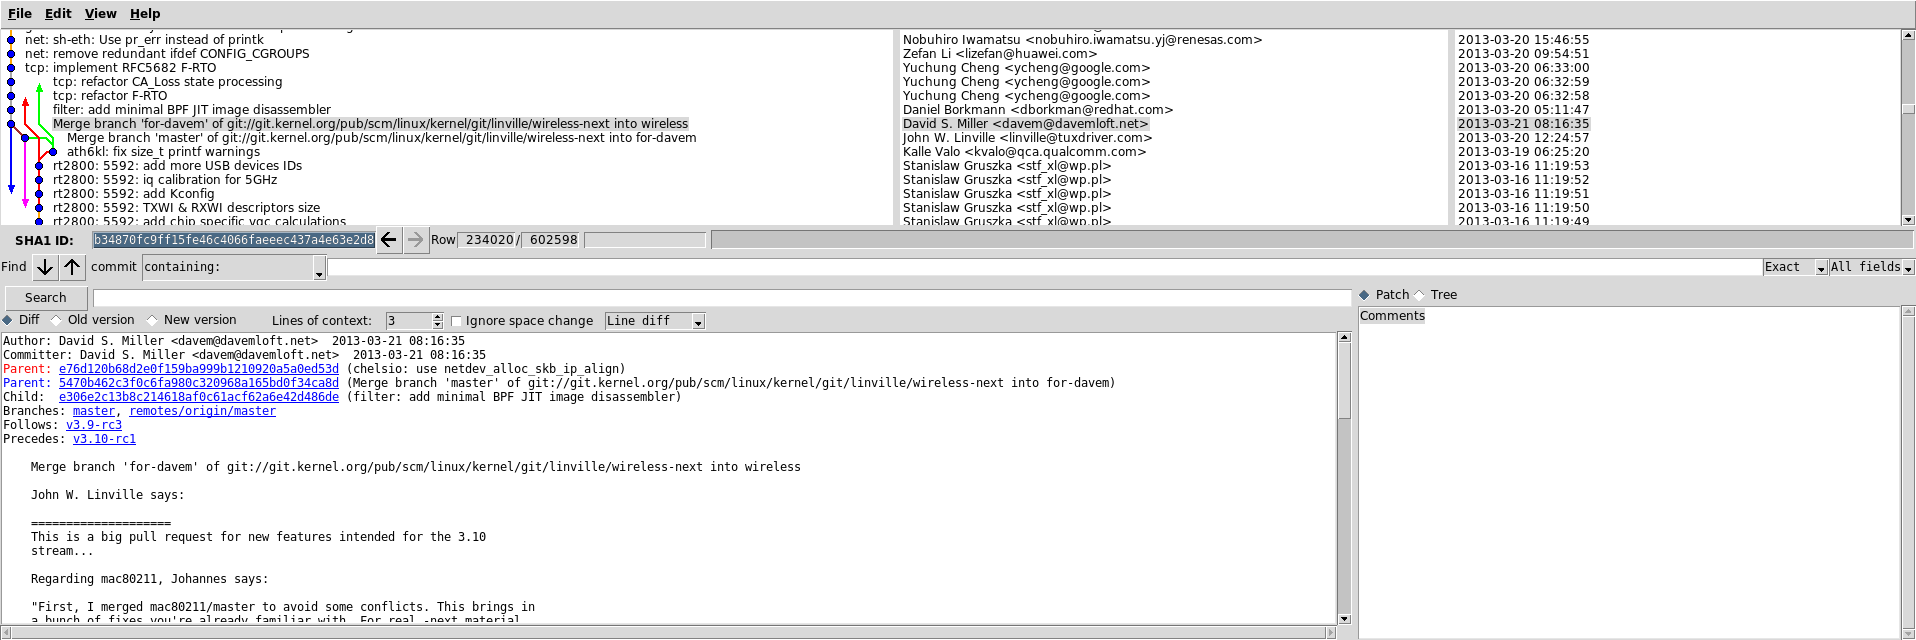
\includegraphics[width=0.47\textwidth]{figures/gitk.png}
        \caption{A sample DAG view of commits from Linux in Gitk}
        \label{fig:gitk}
\end{figure}

Git cannot store the date that a commit was merged into a branch due to the rebase
operation. A rebase can perform serveral changes to commits and merges. It may be
squashed with other commits, combining the effects of several commits into a single
commit. It may be dropped altogether, in which case the commit is no-longer merged.
It may be that the entire branch has simply been re-rooted to another position on
the DAG. Due to this, tools are unable to determine when a commit is merged. A user
may decide that it is important to be able to see only the commits contributing to a
given release, that is commits that were merged with the Linus-branch of the kernel
between two given dates. This operation is not possible without the collection of
additional data that is not provided by git. Git only enables users to see when a
commit was authored, not when it was merged into a branch.

German et al. recorded the metadata of every commit and merge in the Linux git
repository starting in 2011 \cite{German2015}, including chronological data that is
not stored by git. We are able to use this information to determine when a commit
has been merged into the kernel, regardless of rebases preceding and proceeding that
point in time. This information is then converted by a heuristic method, described
by German, to generate sets of trees, which we use as our core model instead of
using the DAG. Each tree is rooted by the top-level merge performed by Linus, which
merges the branches or a set of commits into the kernel.

In this paper, we present our design decisions behind a web-based
tool\footnote{\url{http://li.turingmachine.org}} built around the tree-based model
instead of the DAG. Our tool provides information about the location of a given
commit in the respective merge tree, the files edited, the modules edited, and the
commit message for a given commit or merge. The tool allows users to apply various
filters, including the release version, along with a keyword or phrase from the log
preview, the name of the author, or the commit id. The user can request all the
root-level merges containing a commit or merge that matches the query, or all
commits and merges that match the query.

Using the tree provides many advantages to the DAG model, but there are two
drawbacks. The first drawback is that a server must query the state of the master
repository since time information is not stored by git. The second drawback is that
the tree construction is a heuristic approach, and in some cases may break.

Our core model provides advantages to the DAG model used by other tools. We separate
the commits and merges into sub-trees and focus on a single sub-tree at a time. This
enables us to filter out commits and merges that do not pertain to the component of
the kernel that we are interested in, providing a clearer picture of what is
happening in a given merge. The tree model also enables us to aggregate metadata
easily. With the addition of the continuous polling of the repository, the model
provides us with a mechanism of performing date-range queries with meaningful
results.

\section{Related Work}

To our knowledge, we know of no git repository visualization systems that build
trees from the DAG provided by git. This may be because more information is required
to generate the trees than what is stored by git. Git uses a DAG model, which
enables history-altering actions, like rebases to occur, whereas older tools like
CVS and svn construct trees\cite{CVS2008} but do not work with history-altering
actions.

A server must sit and monitor the git repository as it changes over time to handle
the changes to history. Many of the visualization tools are designed for a
general-purpose approach, where any repository is directly usable without additional
information. Polling for this additional information makes the visualizer specific
to a repository or project.

\subsection{Other Visualizers}

Gitk, Gitg, and other similar git repository visualization tools use the DAG as the
central organization model. This model is sufficient for smaller projects, providing
meaningful information; however, in larger projects, like the Linux kernel, the
branches become too tangled and too deep to derive any meaning from the DAG. Users
can interact with the DAG by going to the previous commit in the chain or jumping to
the parent merge. This suggests that Gitk and similar tools are designed for users
working from a given commit or leaf-node toward the root. With this model, it is
difficult for users to see what other commits are involved with a given merge.

Furthermore, the DAG model is only able to provide file-level information for
commits. It is unable to quickly aggregate the file data over all commits that
are part of a merge. If a user would like to view what files were edited at a merge,
they must manually aggregate this information by hand. While some merges are
relatively small, containing less than 10 commits, other merges are large,
containing over 1500 edited files, as in the case of commit \textit{73287a4}. This
issue is important for authorship and licensing. A merge can only show one author,
the contributor making the merge, but does not show who wrote the commits contained
within that merge.

\begin{figure}
        \centering
        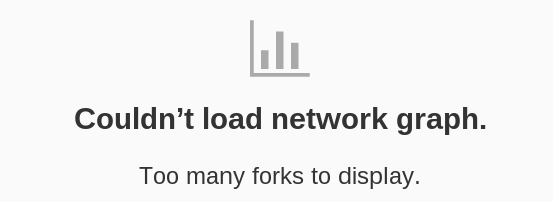
\includegraphics[width=0.45\textwidth]{figures/github_viewer.png}
        \caption{Github Failure Message showing the DAG of the Linux Project}
        \label{fig:gitfail}
\end{figure}

%% Check for papers if they exist
%% This tool isn't specifically designed for showing Linux

\subsection{Treemap visualizer}

University of Maryland presented a treemap visualization
tool\footnote{\url{https://www.cs.umd.edu/hcil/millionvis/Treemap_Visualization_of_the_Linux_Kernel_2_5_33.html}},
pictured in figure \ref{fig:treemap}, for displaying the file structure of a given
version of the kernel. Treemaps are good for visualizing the topology of shallow,
wide trees, making it a good candidate for displaying file systems. Treemaps are
limited in what information can be displayed. The information within the treemap
does not provide clear insight on what changes were made to the files in the given
release, only providing information on where the file is located within the file
system, that is they do no provide temporal information. File systems and the merge
tree of the kernel share many similarities, in both cases, they represent trees that
are wide and shallow, suggesting that a treemap could potentially work to visualize
the commit and merge structure of the kernel.

The treemap is unable to take into account multiple commits behind the same merge
with the same log preview message. Commits and merges have an ordering in which they
were added to the kernel, which cannot be represented by a treemap, but is important
and can be used to assist in building the tree.

The treemap design is also designed for working with data of differing types. In the
filesystem, there are many kinds of files. There are text files, scripts, images,
binary files, and other types. These can be given colours making differences stand
out. There is no obvious way to assign meaningful types to the commits such that all
the commits within a given merge do not all have the same colour, although a user
could be given a controller to colour by author or number of files edited.

Finally, the treemap does not provide any additional information about the
contents of each cell, only that the cell exists and where it exists in the
tree. The user is unable to see their current position within the map, or if we
assume that their current position is the largest surrounding box, they can
no longer see how their current position interacts with the rest of the
system.
%% https://www.cs.umd.edu/hcil/millionvis/Treemap_Visualization_of_the_Linux_Kernel_2_5_33.html
%% Find paper for this maybe?

\begin{figure}
        \centering
        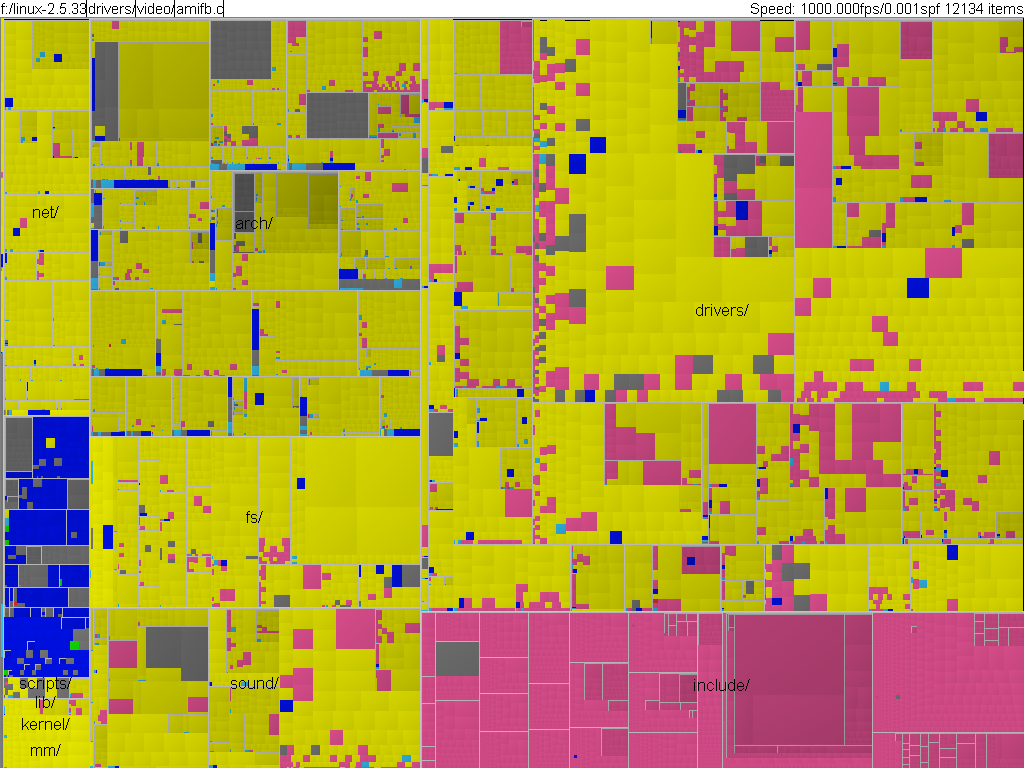
\includegraphics[width=0.47\textwidth]{figures/kernel-files.png}
        \caption{Treemap of Linux 2.5.33 file structure}
        \label{fig:treemap}
\end{figure}

\subsection{List viewer}

Moghaddam designed a web-based visualization
tool\footnote{\url{http://web.uvic.ca/~arasbm/gitVisualizations/linuxRGraph.html}}
displaying the chain of merges into the kernel. There is no information on what
commits are within a given merge, or what files were edited. The visualization
tool provides information about who authored the commit and when it was
authored. We can see the visualization tool in figure \ref{fig:listviewer}
displaying a part of the kernel commit information, from commit ``26b23ac''
according to the tool.

%% http://web.uvic.ca/~arasbm/gitVisualizations/linuxRGraph.html
%% Find paper for this maybe?

\begin{figure}
        \centering
        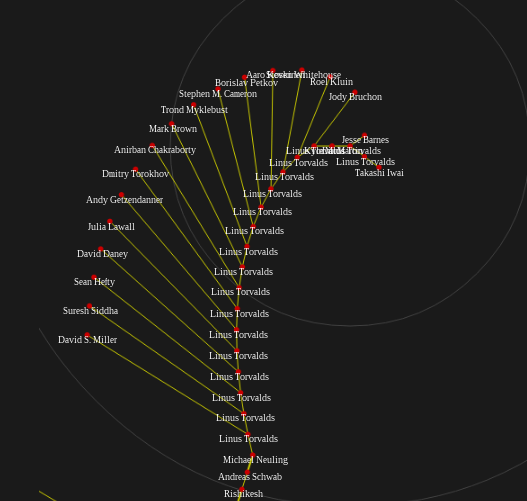
\includegraphics[width=0.47\textwidth]{figures/gitvis.png}
        \caption{List Viewer}
        \label{fig:listviewer}
\end{figure}

\section{Methodologies}
\evan{Correct section title? Other than just trying stuff, what were the
methodologies?}

The goal is to build a tool that makes navigation of the kernel commit information
simpler, while providing an explanation of the changes occurring at each commit and
merge. We designed the tool with two use-cases in mind, though a user may switch
between the cases as they work.

\textit{Use-case 1: top-to-bottom approach}\label{sec:usecase1}\\
These are users that are maintaining a section of the kernel and would like to pick
a merge and merge it directly into their current repository, which is useful for
reducing the amount of re-implementation work. For them, it is important to have the
ability to aggregate metadata about files and modules being effected by the merge.
It is also important for them to be able to navigate from the root toward the
leaves.

\textit{Use-case 2: bottom-to-top approach}\label{sec:usecase2}\\
These are users that start with a known merge or commit and would like to see what
other changes are being made in commits that are in the same merge. This is useful
to see how changes in a given file will break other changes made in the surrounding
commits in the same merge. This is primarily for maintainers that need to perform
some implementation work in order to correctly merge patches from the future. We
must provide these users a mechanism for navigating from a single commit toward the
root, allowing them to see the bigger picture.

\subsection{Core Model}

We root the tree with the merge made by Linus. Each merge may contain zero or more
children, which are other merges and commits. If a merge is cherry-picked or rebased
there will be no children as this information is lost when the rebase occurs.
Commits have no children and are always leaf nodes. The commits contains the
metadata for the changes made. This metadata includes the files changed, the lines
added and removed from each file, the author, the date the commit was merged into
the merge that led to being merged into the kernel, and the date the commit was
authored, the diff, and the commit log. Merges contain less metadata, only storing
the author of the merge, the log, the commit date, and the author date. The details
of the model are outlined by German \cite{German2015}.

\section{Design}


We came up with two designs. We recognized that the structure of the repository was
similar to the wide and shallow tree-structure of a file system. We began with a
command-line shell interface. Then transitioned to a web-based tool where we looked
beyond the file system structure. In this section, we describe the progression of
our tool design, showing the benefits and drawbacks of each component.

\subsection{Command-line Shell}

Our initial intuition was to work with the commits and merges as directory trees
where the commits are files and the merges are directories. There are many
similarities between the tree structure of a file system and the tree structure of
the repository. Both trees are generally shallow, but very wide. File systems have
been studied for quite some time and there are many tools capable of visualizing and
working with the file structure.

The first tool we implemented was a small command-line shell (figure
\ref{fig:shell}) that allows users to navigate through the commits and merges as one
might navigate through files and directories. A user could navigate toward the
leaves of the tree by using the \verb|cd| command followed by the commit id of the
next merge. The user could then navigate toward the root by issuing \verb|cd ../|,
as they would in a file system. Users can use \verb|ls| to view what commits and
merges exist in the current working merge, then use \verb|cat| to view the log
preview of a commit or \verb|more| to see the preview and how many lines were added
and removed from the files in the commit.

\begin{figure}
        \centering
        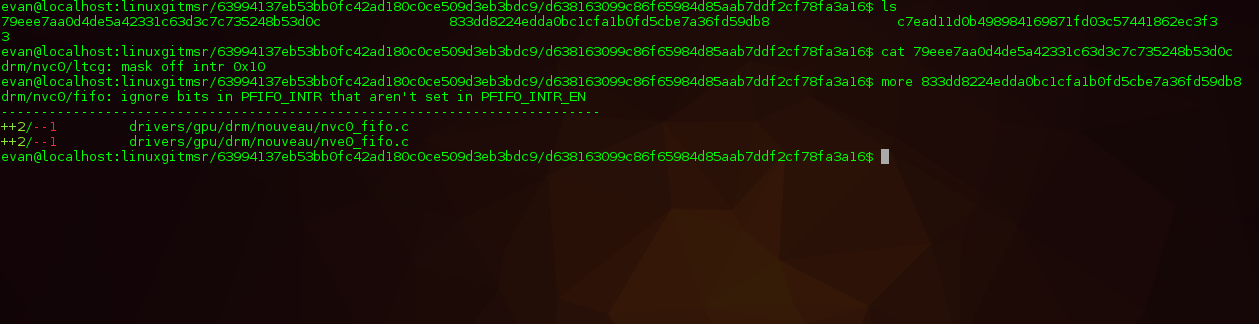
\includegraphics[width=0.47\textwidth]{figures/shell.png}
        \caption{Shell Design}
        \label{fig:shell}
\end{figure}

The shell does not meet our design goals. It only provides users with the ability to
navigate from the root. If there is a commit or merge that they would like to
investigate, they must find it with another tool and navigate through the tree to
find it. Furthermore, it does not aggregate information in the merges, so users must
manually aggregate the metadata. Another issue with this design is that it presents
the users with the commit hashes, which are quite long and unpleasant to remember
and type into the shell, but also do not provide any quick explanation of what the
commit or merge may contain.

\subsection{Web-based Tool}

We replace the command-line interface with a web-based tool. Creating a web-based
tool enables users to use the system without having to install additional software
or carry a large database, making it more accessible, more easily maintainable, and
platform independent. A web-based tool can utilize more interactive means of
navigation and provide better explanations of commits and merges than the
command-line interface.

Our tool uses the following mechanisms to reach our goals of better navigation and
better explanation of the changes.

\begin{itemize}
        \item Filter by search
        \item View files edited
        \item View modules
        \item Tree viewer
\end{itemize}


\begin{figure}
        \centering
        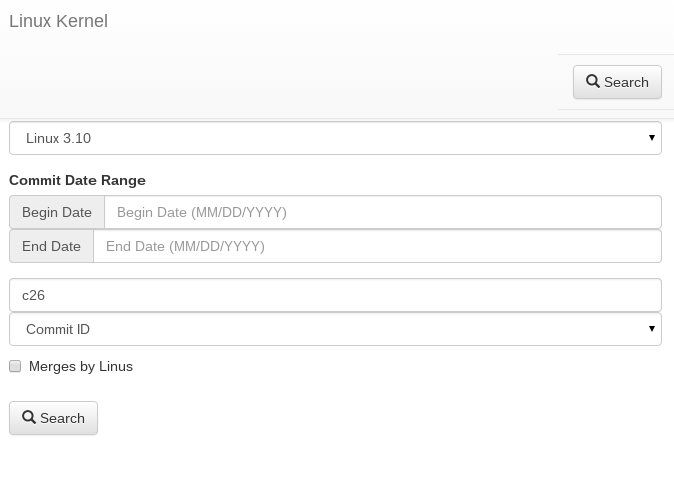
\includegraphics[width=0.47\textwidth]{figures/search.png}
        \caption{Search View}
        \label{fig:search}
\end{figure}

Searching allows a user to filter commits and merges that are irrelevant. The search
mechanism breaks down the results by release version. A user can further narrow down
the search range using the commit date range. The commit date refers to the date of
the creation of the top-level merge. The commits and merges that are returned may
have a commit date beyond the given range if they were merged by Linus within the
date range. A user may then provide a search text, filtering on the author name,
the commit id, or keyword from the log. Any part of the author name may show up in
the results, including searching by email address. The commit ID must be specified
from the first character to the last character. For example, the commit
`c267548755a184ef97301071300c1739a564e135' is returned when the user searches for a
commit id of `c26' in the 3.10 Linux kernel. We will use this commit for showing
each of the features of the tool.

\begin{figure}
        \centering
        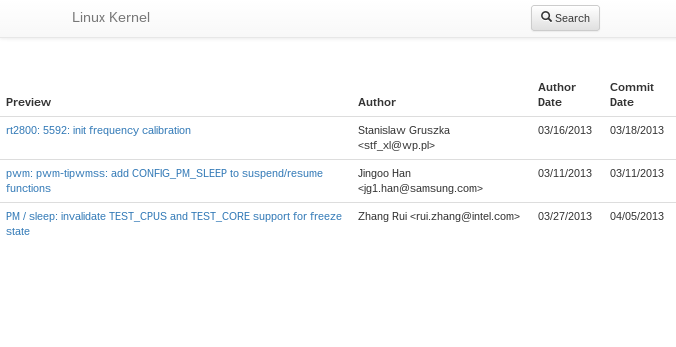
\includegraphics[width=0.47\textwidth]{figures/search_results.png}
        \caption{Search Results}
        \label{fig:results}
\end{figure}

In the search results, the user is presented with the one-line log message preview,
the author's name and email, the date the commit was authored, and the date the
commit was last committed. The commit date and author date will usually be the same;
however, if the commit has been rebased or cherry-picked into a merge that
eventually is merged into the kernel, the commit date and authored date will be
different. We can see this in the first and third entries in figure
\ref{fig:results}.

\begin{figure}
        \centering
        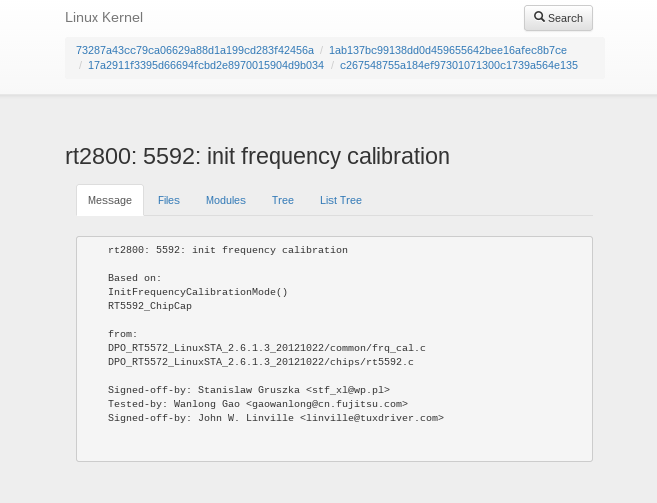
\includegraphics[width=0.47\textwidth]{figures/message_view.png}
        \caption{Commit Message}
        \label{fig:message}
\end{figure}

Once a user selects a commit or merge to investigate, they are presented with a
tabbed pane allowing them to view the full commit log, the files edited, the modules
involved, and the tree views.

The first tab displays the full commit log. From this, a user is able to see what
they would see had they searched for the commit using git log. This doesn't provide
additional information to the other tools, but helps to complete the functionality
of our tool. The commit log provides a user with the information about the content
of the commit and who has signed-off on the commit to ensure that it is good
quality. The message for merges may also contain the information about the commits
that are being merged into a given merge. The information within these messages is
highly variable, and is completely dependent on the author's style. As the user
moves toward the top-level merge, the quality of these messages generally improves.

\begin{figure}
        \centering
        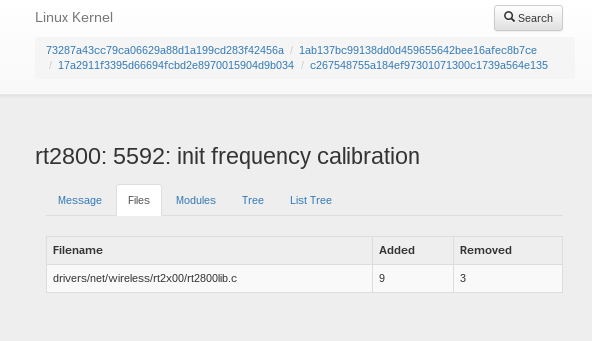
\includegraphics[width=0.47\textwidth]{figures/file_view.png}
        \caption{Commit Files}
        \label{fig:files}
\end{figure}

The second tab is the files tab. This tab provides information on what files have
been edited, how many lines were added, and how many lines were removed in a given
commit. This functionality is similar to the other tools available. Our tree-based
design model allows us to extend this functionality to merges, which the other tools
are unable to show. When a file is edited multiple times from different commits
within a merge, we simply add the added and removed lines to the values already
stored, though this could be extended to use the diff information to determine when
a line has been replaced rather than incrementing the lines removed and the lines
added.

\begin{figure}
        \centering
        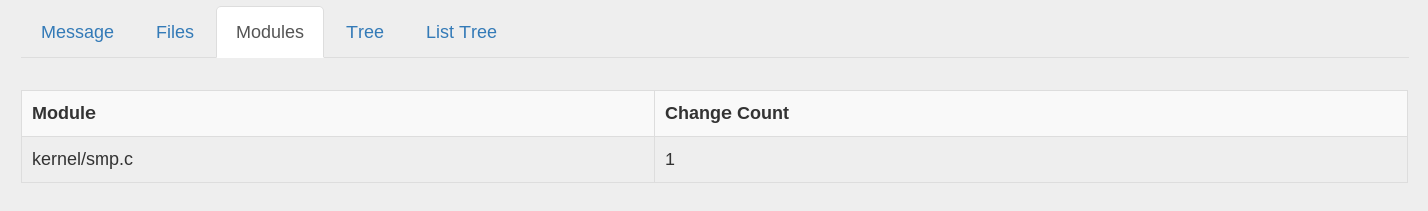
\includegraphics[width=0.47\textwidth]{figures/modules.png}
        \caption{Commit Modules}
        \label{fig:modules}
\end{figure}

The modules tab shows the modules that are contained within the commit. Modules are
not natively recognized by git, and are not going to be present in all repositories.
In the Linux repository, authors put the module they are working on in the one-line
preview of the log-message. We heuristically extract the module by taking all text
in the log preview of commits until the first colon.  Modules are logical partitions
of the information in the kernel. Depending on where the author was working, modules
can be general, such as ``bluetooth'' and ``wireless'', or can be quite specific for
individual hardware, such as ``ath9k\_hw'' and ``wl1251''. In a few cases, the
author of a commit does not correctly follow this format and the hueristic approach
fails. Like files, we are able to show what modules are edited in merges and
commits. The image in figure \ref{fig:modules} shows the modules for a commit. A
commit will only ever have one module that it is associated with, merges with more
than one child will have more.

Finally, we have the tree view tab. The tree view is designed for providing easy
navigation within a tree and providing a clear topological view of the branch off
the kernel. We have experimented with various tree designs to find a design that
allows for easy navigation and visualization of both large and small trees. We
discuss the various tree designs in section \ref{treeview_section}.

\subsection{Tree Views} \label{treeview_section}

The tree view is what makes this tool unique to other tools, providing a full view
of the entire merge tree. We have experimented with various types of trees; list
trees are similar to the representation used in many file system explorers,
Reingold-Tilford trees clearly represent the tree structure, and bubble trees
organize the data hierarchically by having the parent node contain the child nodes
similarly to tree maps, but clearly showing the parent-child relationships between
nodes.

\subsubsection{List Tree}

The list tree viewer is in the form of nested lists, and is designed to more closely
model the tree hierarchy view found in file browsers. This tree only contains the
commits and merges that are within the subtrees of the current merge. A commit will
never have any items in this tree as it is a leaf. To accompany the tree, we include
breadcrumbs at the top of the page to enable a user to navigate both from the root
to the leaves and from a leaf to the root. The last item in the breadcrumb list is
the current commit, the previous item is the parent of the current commit, and the
first item is the root merge into the kernel.

\begin{figure}
        \centering
        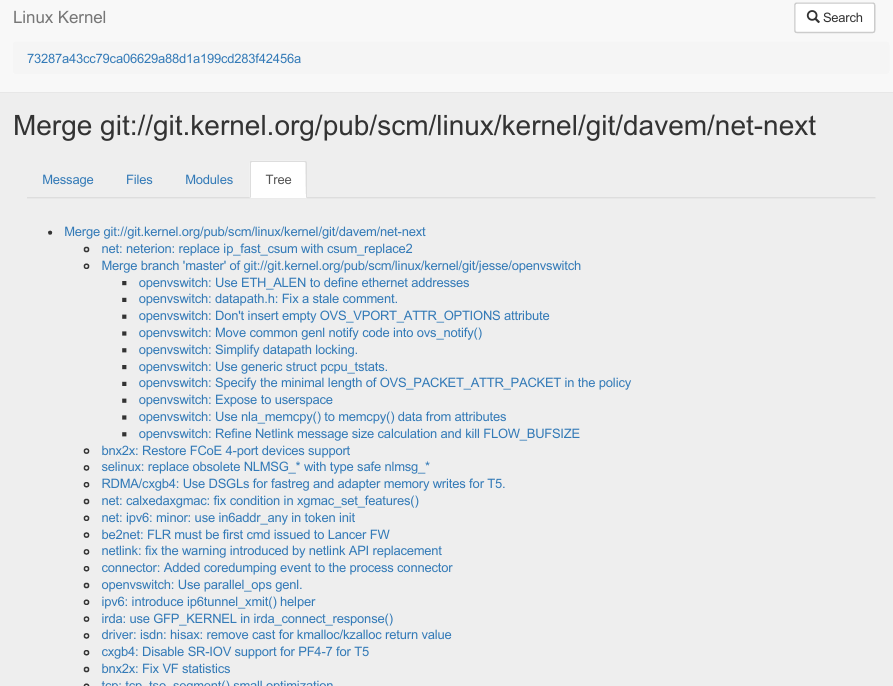
\includegraphics[width=0.47\textwidth]{figures/list_tree.png}
        \caption{List Tree}
        \label{fig:list_tree}
\end{figure}


\subsubsection{Reingold-Tilford Tree}


The Reingold-Tilford tree produces very nice results, creating an intuitive
representation of the tree. The representation has a clear notion of root and
leaves, and how to navigate in either direction.

\begin{figure}
        \centering
        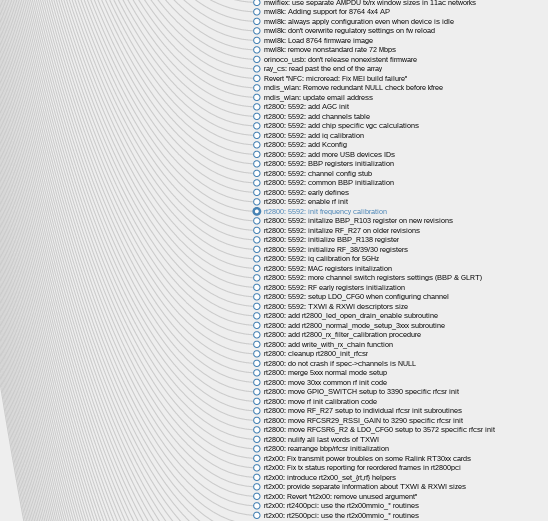
\includegraphics[width=0.47\textwidth]{figures/tree_view.png}
        \caption{Reingold-Tilford Tree}
        \label{fig:tree}
\end{figure}

Clicking on subtrees will cause them to minimize, only showing parts of the tree
that are of interest to the user. Furthermore, the user can zoom the tree by
scrolling the mouse wheel to see more of the topology of the tree, or to see the
details of a given part of the tree.

Some of the merge trees are very large (figure \ref{fig:zoomed_tree}), containing
thousands of commits and merges. While the tree is capable of producing a
visualization, it becomes much more difficult to understand.

\begin{figure}
        \centering
        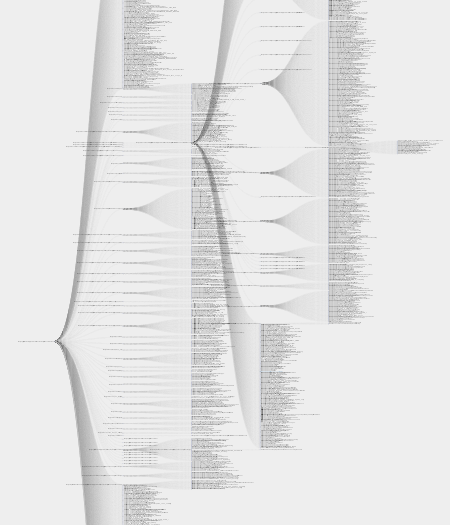
\includegraphics[width=0.47\textwidth]{figures/tree_zoom.png}
        \caption{Reingold-Tilford Tree zoomed out}
        \label{fig:zoomed_tree}
\end{figure}

\subsubsection{Bubble Tree}

The bubble tree provides a very clear picture of where a commit is located in the
hierarchy. The currently selected commit or merge is colored red, while non-selected
merges use a shade of blue and commits use white. The depth of the blue colouring is
dependent on how deep in the hierarchy that node is. The root is the lightest blue,
and the contained merges are progressively darker.

\begin{figure}
        \centering
        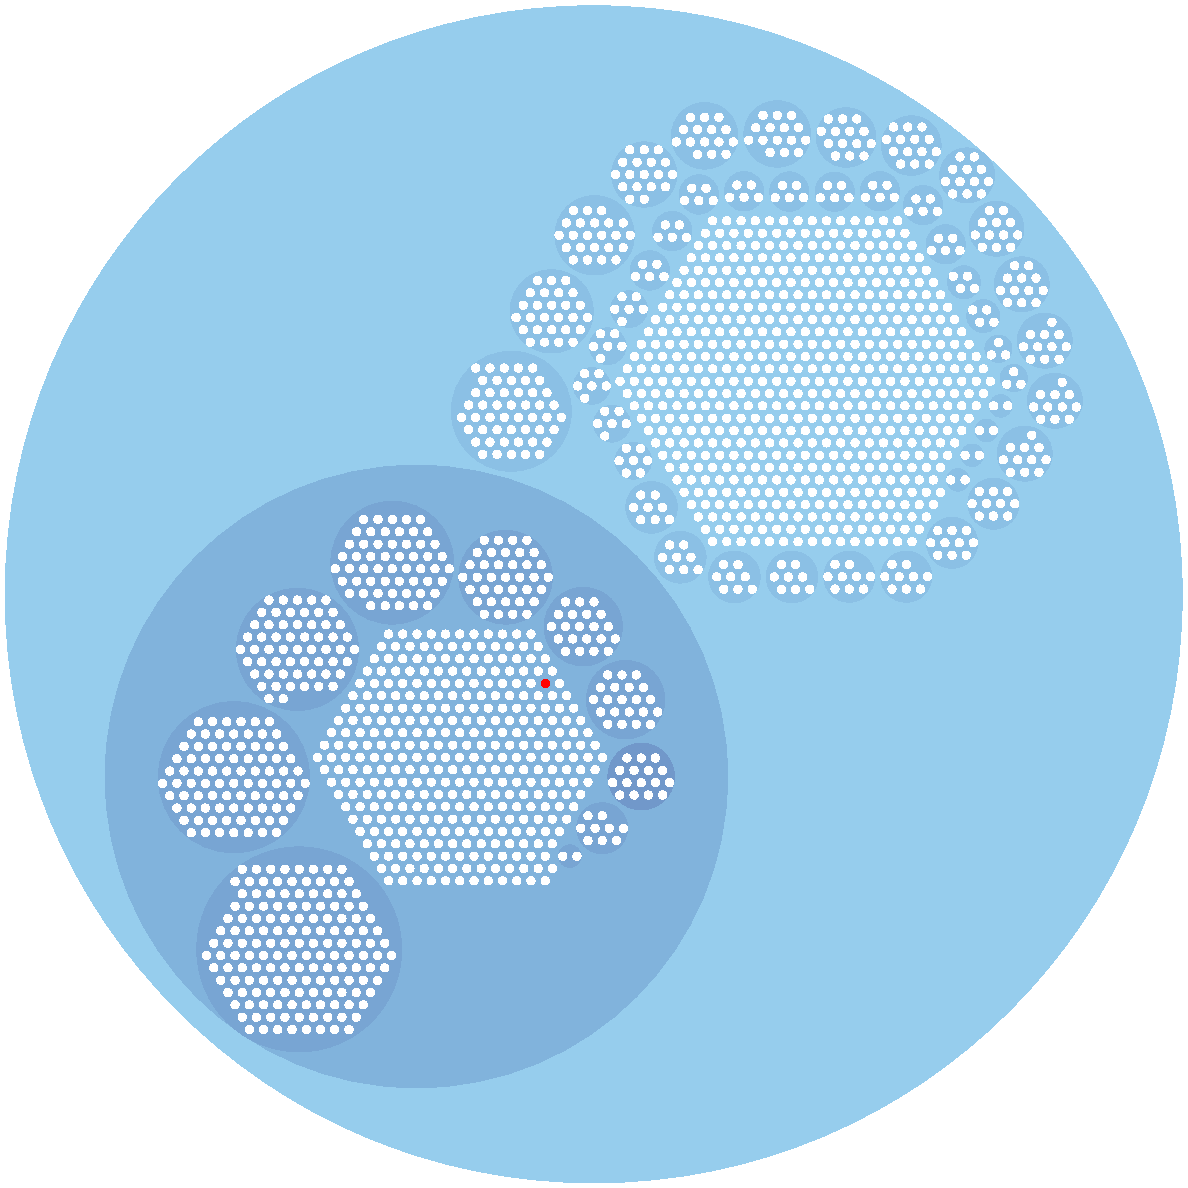
\includegraphics[width=0.47\textwidth]{figures/bubble_tree.pdf}
        \caption{Bubble Tree}
        \label{fig:bubble_tree}
\end{figure}

The bubble tree doesn't have an implicit way of providing additional information,
placing any text near the nodes makes the tree impossible to read, so we include a
separate pane in the web page. When a user hovers over a node, the pane shows
additional information about the author and the commit message and a link to the
detailed page for that commit or merge. If the user clicks on a node, the tree will
zoom to that node and the information in the info pane will persist, enabling the
user to click the link. This tree provides an easy mechanism for users to navigate
from the root to the leaves and vice versa.

\section{Implementation Details}

\evan{Is this section necessary?}

We built a web-based tool to provide information about the kernel.  We chose to use
Nginx as the main web server, postgresql as the dbms, and Flask as the framework for
generating the dynamic content.

Nginx is a high-performance, scalable HTTP and mail server. Started in 2002, the
project is much younger than the Apache project, and designed with massive
scalability and multi-processing in mind. Instead of using request-driven threading,
Nginx uses an event-driven architecture, making it more scalable, proving itself as
being the web server behind large sites like Netflix, Hulu, GitHub, Tumblr, and many
other popular sites\footnote{\url{http://wiki.nginx.org/Main}}.

Postgresql is our dbms of choice, providing fast and reliable results. There are
multiple reasons behind choosing postgresql over another dbms. The main reason being
that the dataset built by German et al. was generated from a postgresql database,
allowing us to import the data directly without any further conversions. The
secondary reason is that we are more familiar with postgresql than the other systems
available.

We chose the python micro-framework
Flask\footnote{\url{http://flask.pocoo.org/docs/0.10/}} for generating the dynamic
content. Working with flask is simple and easy, allowing us to work in Python.

The database itself is broken down into 5 main tables; commits, filesmod, logs,
pathtomerge, and releases. Commits contains most of the metadata for each commit, it
contains the author, the authored date, and committer, the commit date, a boolean
saying what is a merge, and the diff. Filesmod contains the information on what
files were modified for the commits. Since a file may be modified by multiple
commits, and a commit may be modifying multiple files, we can do one of two things
for the primary key. We could use both the filename and the commit id as the primary
key, but we just use an index. The filesmod table contains the filename, the commit
id, the number of lines added, and the number of lines removed. Trivially, it
contains the index, but that isn't necessary for anything beyond the primary key.
Logs contains the information for each commit log, this is the one-liner preview
message and the full message. Pathtomerge is the important table. Pathtomerge
contains the commit id, the number of merges between the commit and the top-level
merge with the kernel, the next merge in the merge path up to the top-level merge
with the kernel, the top-level merge into the kernel, and when it get merged into
the kernel. The information in this table must be generated periodically by the
server because we are unable to generate the tree structure correctly straight from
the information stored by git. Pathtomerge does not contain any top-level merges, as
these will never have a next merge in the tree, since we are only storing the
parents and not the children, storing the top-level merge is redundant and
unnecessary. The releases table stores the release information.  It contains the
version name, whether the version is a candidate release or a real release, the
previous version, the previous non-candidate release version the previous version
commit id, the previous non-candidate release version commit id, and the commit id
of this version. The version commit id represents the last top-level merge into the
version of the kernel. Using this and the commits table, we are able to determine
the release date of any version of the kernel. Then using the previous release date,
we can find the range of dates where valid top-level merges are found for that
version.

\section{Discussion}

Our tool provides mechanisms and visualizations that other tools are unable to
produce. Continuous mining of the repository\cite{German} provides more information
about how the repository is changing. It gives us the ability to see how commits are
being merged into the kernel, allowing us to more reliably build trees from the
snapshots of the repository.

\begin{figure}
        \centering
        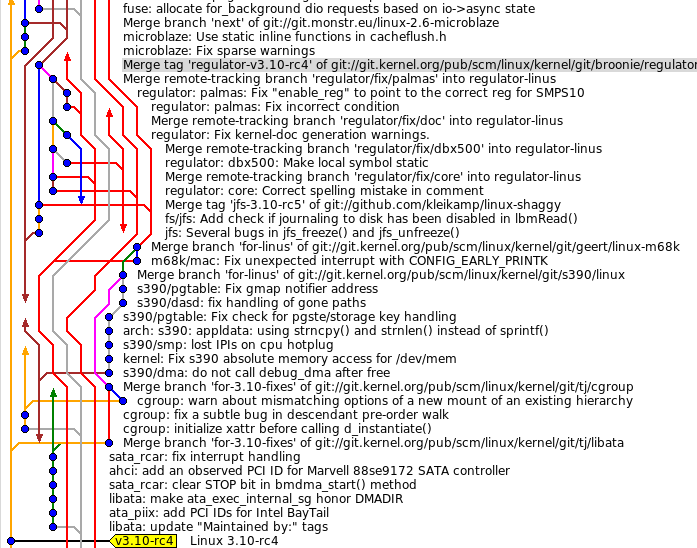
\includegraphics[width=0.47\textwidth]{figures/042dd_DAG.png}
        \caption{Merge Dag View}
        \label{fig:dag_view}
\end{figure}

\begin{figure}
        \centering
        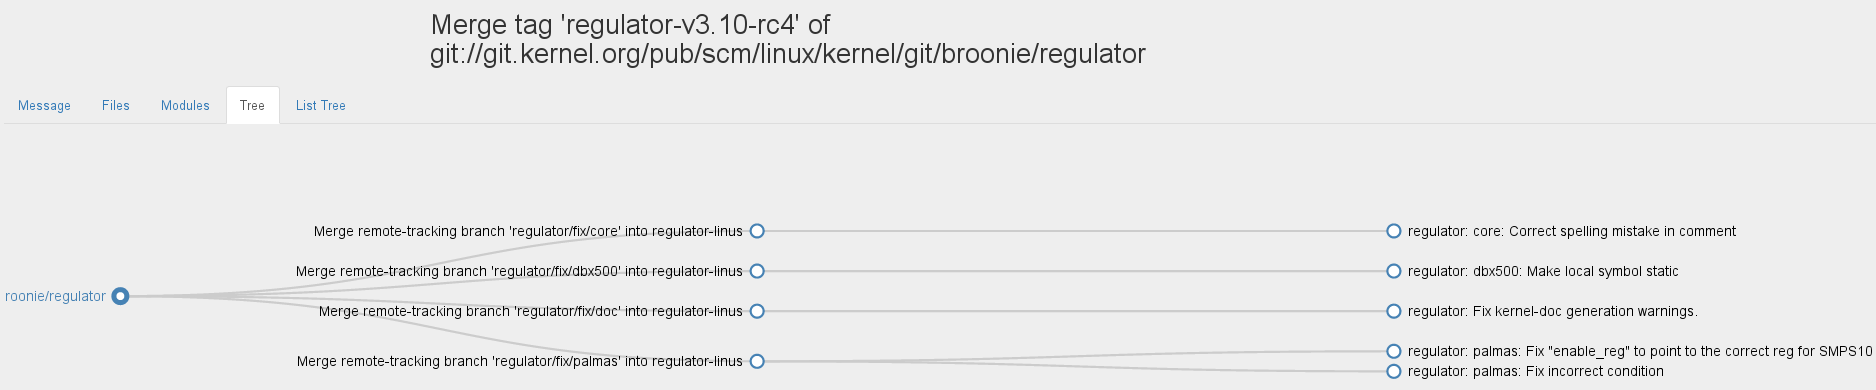
\includegraphics[width=0.47\textwidth]{figures/042dd_tree.png}
        \caption{Merge Tree View}
        \label{fig:tree_view}
\end{figure}

Our goal was to build a tool to enable maintainers to effectively navigate and
pull explanation of the changes performed to the kernel over the period of a
release. Achieving this goal includes removing information that does not
pertain to given users. In figure \ref{fig:dag_view} and figure
\ref{fig:tree_view}, we can visually compare the results returned from gitk and
our tool for the top-level merge ``042dd60ca6dec9a02cefa8edd67de386e35755d6''
from kernel version 3.10. The relevant information in both of these figures is
identical, but the presentation drastically changes our ability to comprehend
what we are seeing. The primary difference is the removal of irrelevant
information. In gitk (\ref{fig:dag_view}), the visualization results include
commits and merges from other components of the kernel, while our tool
(\ref{fig:tree_view}) only includes the results that are specific to the
component of the kernel that we are interested in.

This merge is relatively small, containing only four merges, three of which
only contain a single commit, and the last containing two commits. With our
tool, we are able to immediately see what commits and merges pertain to our
section of the kernel. The DAG view of this provides almost no explanation,
furthermore, users must work to determine where this merge ends and the next one
begins.

Our tool further enhances our understanding by immediately giving us the files
and modules that were edited in the branch. We are able to determine that three
files, ``palamas-regulator.c'' had two lines added and two lines removed,
``dbx500-prcmu.c'' had 12 lines added and 12 lines removed, and ``core.c'' had 5
lines added and 2 lines removed. Finally, we are able to determine that only the
``regulator'' module was modified in this merge and was modified by 5 commits.

\subsection{Extendability}

The front-end uses asynchronous requests to gather the information for the trees and
tables. This enables third-parties to implement new front-ends, trying other
designs, though this interface may change in the future. The tree, file, and module
information is accessible through 
http://li.turingmachine.org/data/tree/JSON/\verb|<commit id>|,
http://li.turingmachine.org/data/files/JSON/\verb|<commit id>|,
http://li.turingmachine.org/data/modules/JSON/\verb|<commit id>|, respectively.

The response for the tree is a single object. This object is the root node of the
tree, and may contain an object of children objects in the \verb|children| field,
which are in the same format as the root object. The children object uses the commit
id as the key.

The tree node objects have the following fields:

\begin{tabular}{ccl}
        Field name & Data type & Description\\\hline
        cid & string & Commit id\\
        name & string & One-line log preview\\
        mlinus & string & Root merge commit id\\
        author & string & Author name and email\\
        mnext & string & Parent merge commit id\\
        children & object & Object of tree objects\\
\end{tabular}

The file responses contain only the files that the selected merge or commit works
with. The response is a single object in the form of a tree. This object is the root
of the tree, and represents the current merge or commit. If the current position in
the tree is an inner node, the response will contain the child nodes in the
``children'' field, otherwise ``children'' will be an empty list. The full response
format for the file response looks like:

\begin{itemize}
        \item ``cid'': string, commit id
        \item ``files'': list, list of tuples in the format
                \begin{enumerate}
                        \item Filename: string
                        \item Lines added: unsigned integer
                        \item Lines removed: unsigned integer
                \end{enumerate}
        \item ``mnext'': string, the commit id of the next merge toward the
                top-level merge
        \item ``children'': list, List of all child objects with the same
                fields. Null if no children.
\end{itemize}

\section{Future Work}

There are still many areas that can be improved before the full potential of our
model can be realized. Here, we outline various areas that still need more
attention.

\subsection{Files}

There is currently no functionality surrounding searching by filename. Use-case 2
may know what file they are editing and try to determine how it may work with the
other commits and merges in the module. It is possible that a third use-case may
arise, where the user wants to determine all commits that effect a given file. In
both cases, a bottom-to-top approach is used. With this functionality, implementing
the top-to-bottom search feature becomes trivial.

There is limited functionality to the presentation of the file information. At a
minimum, the patches for the commits can be displayed. From there, the patches can
be used to piece together parts of the file to generate a single patch at a given
merge rather than displaying each patch individually. The patches can also be used
for determining what kinds of changes were made, if the lines are being added,
removed, or replaced.

\subsection{Authorship}

Our model can aggregate more information than what we have implemented. The
authorship information is important for licensing purposes, and we can show all
authors contributing to a merge and how many commits they contributed to the merge.
We could go further, providing information about what files they edited, how many
lines they added and removed, and more.

\subsection{Diff generation}

Due to the construction of the tree, it is possible to generate a diff of a given
file in a merge. This would remove areas that overlap, and provide users with a
single patch at a merge rather than attempting to combine all of the diff files from
the leaves.

\subsection{Evaluation}

At this time, we have no evidence that our tool is able to improve the work-flow of
maintainers. We believe that the tool is able to improve the work-flow and
performance of maintainers because it provides cleaner mechanisms of visualizing and
presenting the commit information. It is able to provide more relevant information,
while removing information that is irrelevant to a given module or set of merges.

We can either perform user-testing to show how a users workflow changes, or we could
have maintainers evaluate and critique the tool and use their feedback to determine
if the tool meets our goals.

\section{Conclusion}

Our tool shows promising results, providing a clearer picture of the relation
between the merges and commits when compared to DAG-based models. Not only are
we provide a clearer visualization, we provide information about the files
edited by all of the commits contained within a merge, and we provide the
information about what modules are edited in a merge.

While we are able to generate a better explanation of the changes happening at
each commit and merge, the tree-model requires more information than what is
provided by git, requiring a central server to monitor changes to the project.
This breaks the design goals of decentralized version control systems and makes
the tool specific to the project.

A tree-based model appears to be sufficient for creating a clean visualization
and explanation of the changes in the Linux kernel.

\nocite{*}
\bibliographystyle{plain}
\bibliography{citations}

\end{document}
